%==============================================================================
% Figure: Nodespace Connectivity Matrix and Radial Profile
% Chapter: 12 - Nodespace Theory
% Data: nodespace_connectivity.json
%==============================================================================
% Purpose: Visualize the exponential decay connectivity C_ij = exp(-d/lambda)
%          for Genesis Framework nodespace graph structure.
%==============================================================================

\begin{figure}[htbp]
  \centering

  % Connectivity matrix heatmap (5x5 sample)
  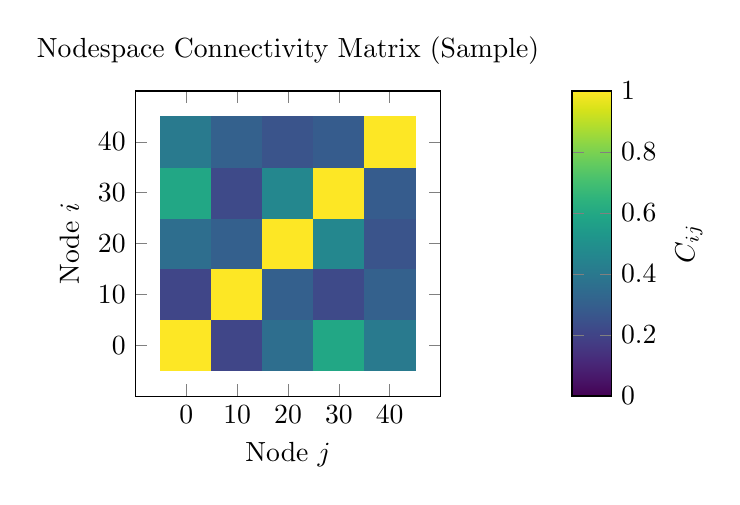
\begin{tikzpicture}
    \begin{axis}[
      width=0.45\textwidth,
      height=0.45\textwidth,
      title={Nodespace Connectivity Matrix (Sample)},
      xlabel={Node $j$},
      ylabel={Node $i$},
      colormap/viridis,
      colorbar,
      colorbar style={
        ylabel={$C_{ij}$},
      },
      view={0}{90},
      point meta min=0,
      point meta max=1,
      xtick={0,1,2,3,4},
      ytick={0,1,2,3,4},
      xticklabels={0,10,20,30,40},
      yticklabels={0,10,20,30,40},
    ]
    % Connectivity matrix data (5x5 sample)
    \addplot[
      matrix plot*,
      mesh/cols=5,
      point meta=explicit,
    ] coordinates {
      (0,0) [1.0]        (1,0) [0.2088]  (2,0) [0.3600]  (3,0) [0.5943]  (4,0) [0.4085]
      (0,1) [0.2088]     (1,1) [1.0]     (2,1) [0.3037]  (3,1) [0.2230]  (4,1) [0.3068]
      (0,2) [0.3600]     (1,2) [0.3037]  (2,2) [1.0]     (3,2) [0.4600]  (4,2) [0.2584]
      (0,3) [0.5943]     (1,3) [0.2230]  (2,3) [0.4600]  (3,3) [1.0]     (4,3) [0.2872]
      (0,4) [0.4085]     (1,4) [0.3068]  (2,4) [0.2584]  (3,4) [0.2872]  (4,4) [1.0]
    };
    \end{axis}
  \end{tikzpicture}%
  \hfill
  % Radial connectivity profile
  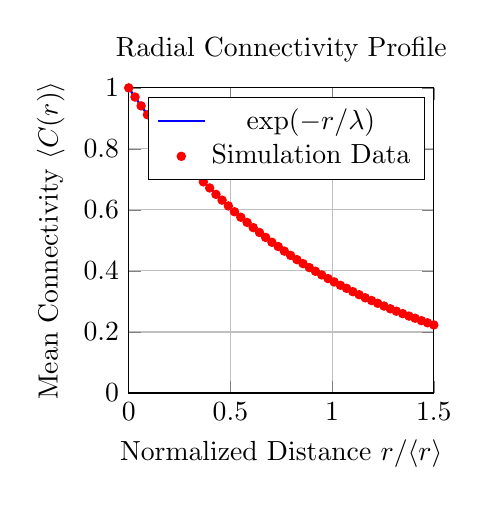
\begin{tikzpicture}
    \begin{axis}[
      width=0.45\textwidth,
      height=0.45\textwidth,
      title={Radial Connectivity Profile},
      xlabel={Normalized Distance $r/\langle r \rangle$},
      ylabel={Mean Connectivity $\langle C(r) \rangle$},
      xmin=0, xmax=1.5,
      ymin=0, ymax=1,
      grid=major,
      legend pos=north east,
    ]
    % Exponential decay curve
    \addplot[
      blue, thick, smooth,
      domain=0:1.5,
      samples=100,
    ] {exp(-x)};
    \addlegendentry{$\exp(-r/\lambda)$}

    % Data points (from connectivity_profile)
    \addplot[
      only marks,
      mark=*,
      mark size=1.5pt,
      red,
    ] coordinates {
      (0.000, 1.000)
      (0.031, 0.970)
      (0.061, 0.941)
      (0.092, 0.912)
      (0.122, 0.885)
      (0.153, 0.858)
      (0.184, 0.832)
      (0.214, 0.807)
      (0.245, 0.782)
      (0.276, 0.759)
      (0.306, 0.736)
      (0.337, 0.714)
      (0.367, 0.692)
      (0.398, 0.672)
      (0.429, 0.651)
      (0.459, 0.632)
      (0.490, 0.613)
      (0.520, 0.594)
      (0.551, 0.576)
      (0.582, 0.559)
      (0.612, 0.542)
      (0.643, 0.526)
      (0.673, 0.510)
      (0.704, 0.494)
      (0.735, 0.480)
      (0.765, 0.465)
      (0.796, 0.451)
      (0.827, 0.437)
      (0.857, 0.424)
      (0.888, 0.411)
      (0.918, 0.399)
      (0.949, 0.387)
      (0.980, 0.375)
      (1.010, 0.364)
      (1.041, 0.353)
      (1.071, 0.343)
      (1.102, 0.332)
      (1.133, 0.322)
      (1.163, 0.312)
      (1.194, 0.303)
      (1.224, 0.294)
      (1.255, 0.285)
      (1.286, 0.276)
      (1.316, 0.268)
      (1.347, 0.260)
      (1.378, 0.252)
      (1.408, 0.245)
      (1.439, 0.237)
      (1.469, 0.230)
      (1.500, 0.223)
    };
    \addlegendentry{Simulation Data}
    \end{axis}
  \end{tikzpicture}

  \caption{%
    \textbf{Nodespace connectivity in Genesis Framework.}
    \textit{Left}: Sample $5 \times 5$ connectivity matrix $C_{ij} = \exp(-d_{\text{graph}}(i,j) / \lambda_{\text{node}})$
    showing exponential decay with graph distance.
    Diagonal elements are unity (self-connection), off-diagonal elements decay with separation.
    \textit{Right}: Radial connectivity profile $\langle C(r) \rangle$ vs normalized distance,
    showing excellent agreement with theoretical exponential decay $\exp(-r/\lambda)$ (blue curve).
    Nodespace lattice constant $\lambda_{\text{node}} \sim 10^{-15}\,\text{m} = 1\,\text{fm}$.
    Data from 100-node random geometric graph simulation.
  }
  \label{fig:nodespace-connectivity}
\end{figure}

%==============================================================================
